Le projet \textsc{UPSimulator} a pour objectif de développer un simulateur de microprocesseur à visée pédagogique. Celui-ci doit permettre d'appréhender la chaîne conduisant d'un programme écrit dans un langage de haut niveau au détail de l'exécution à l'échelle du processeur. Pour cela, le projet doit permettre:
\begin{itemize}
	\item la production d'un code source dans un langage jouet;
	\item la compilation du code source et la production d'une version assembleur et binaire de celui-ci. Le simulateur doit permettre l'usage de différents modèles (taille des mots binaires, nombre de registre, ...);
	\item le suivi de l'exécution (registres, mémoire, pointeur, appels à l'UAL,...);
\end{itemize}

Les choix techniques retenus pour chaque fonctionnalité sont développés ci-après.

\begin{figure}[h!]
	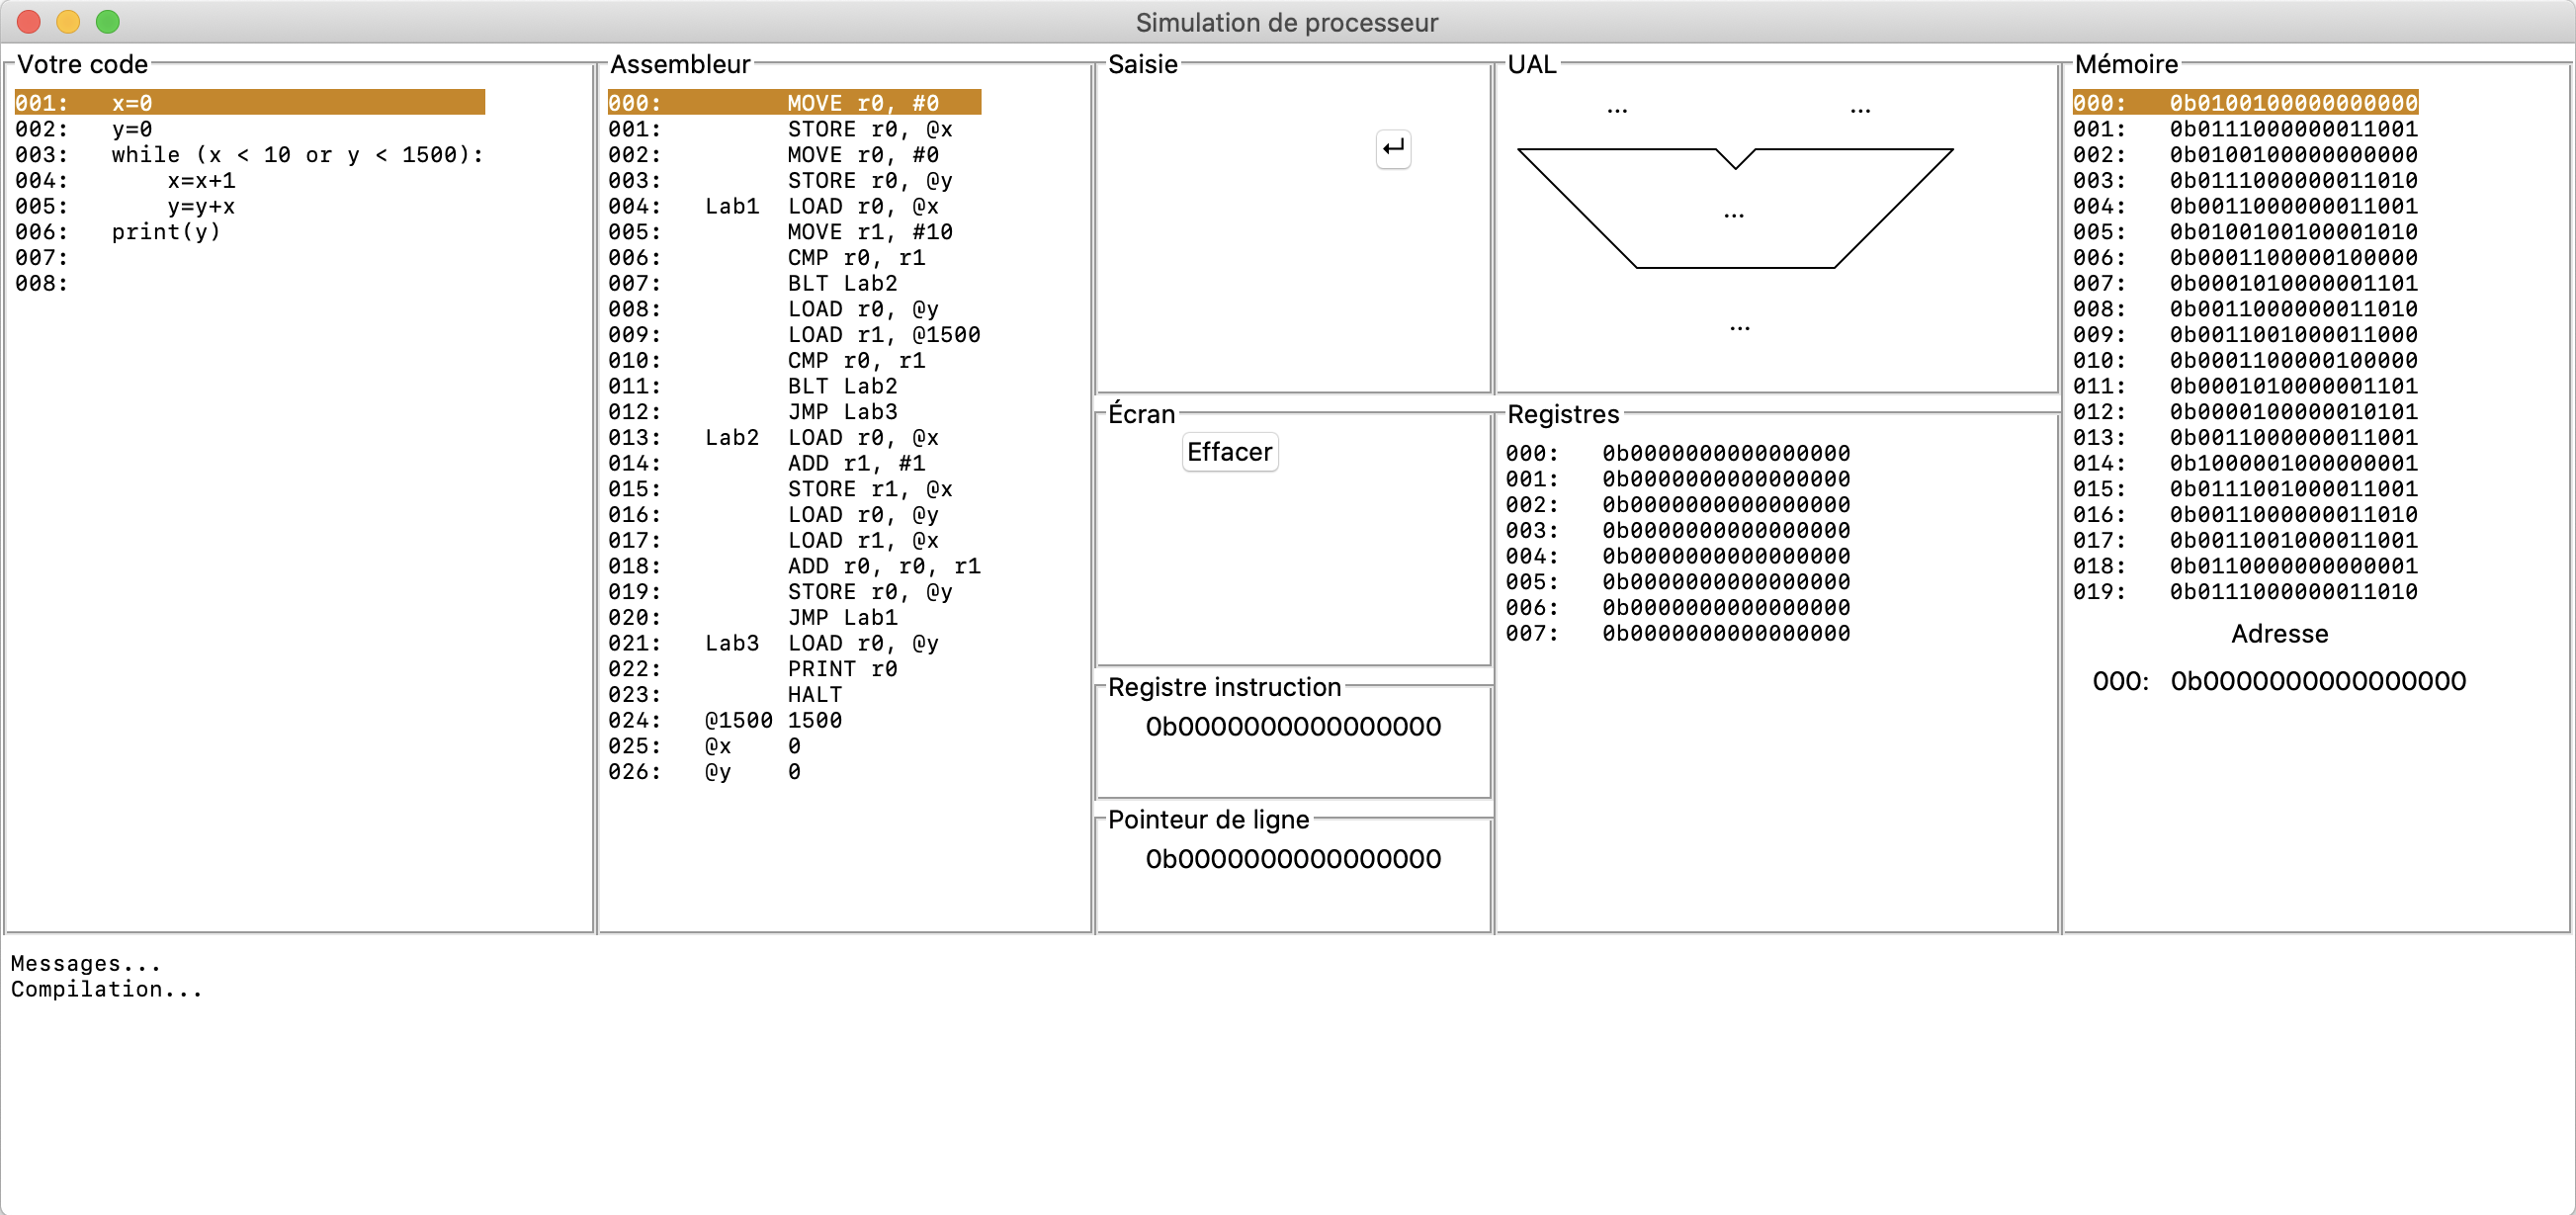
\includegraphics[width=\textwidth]{./Pictures/Header.png}
	\caption{\label{fig:gui} Interface Graphique}
\end{figure}

Pour accéder à l'interface graphique: \mintinline{shell}{python uPSimulator.py}